\section{Обзор предметной области}
\subsection{Задача компьютерного зрения}
Компьютерное (машинное) зрение (Computer Vision) – это совокупность программно-технических решений в сфере искусственного интеллекта (ИИ), нацеленных на считывание и получение информации из изображений, в реальном времени и без участия человека. 

Большое количество информации человек получает при помощи зрения. 
Изображения способны хранить огробное количество информации. Как следствие их использование в компьютерных системах способствует увеличению их производительности. Однако такие технологии требуют сложных вычислений. Задачей компьютерного зрения является разработка эффективных алгоритмов, выполняющих извлечение и анализ данных из изображений или видео. 
 
В настоящий момент, такие технологии применяются для решения таких сложных задач как:
\begin{itemize}
    \item OCR – Optical character recognition (Оптическое распознавания символов): преобразование текста на изображении в редактируемый.
    \item Фотограмметрия – технология создания трехмерной модели объекта на основе фотографий, сделанных с различных ракурсов.
    \item Motion capture – технология, широко применяемая в киноиндустрии, позволяющая преобразовывать движения реальных людей в компьютерную анимацию.
    \item Дополненная реальность (AR) – технология, позволяющая в реальном времени проецировать виртуальные объекты на изображение реального окружения. 
    \item Медицинская диагностика – обнаружение раковых клеток на ранней стадии, увеличение качества МРТ изображений, их анализ и т.д.
\end{itemize}
\subsection{Искусственные нейронные сети}

\subsubsection{Понятие искусственной нейронной сети}

Машинное обучение (Machine Learning) – раздел исследований в сфере ИИ, в основе которых лежат методы разработки систем способных к обучению. Алгоритмы машинного обучения эффективно себя показывают в задачах, в которых требуется у заранее подготовленных (обучающих) данных определить общие признаки и по ним идентифицировать новые данные. В формировании таких, обучающихся, систем часто применяют искуственные нейронные сети. 

Искусственная нейронная сеть (ИНС) – компьютерная модель, в основе которой лежат принципы работы биологической нейронной сети - совокупности связанных между собой нервных клеток - нейронов. Каждый нейрон имеет набор входных связей - синапсов, по которым он получает информацию, представленную в виде импульсов, от других нейронов. По полученным данным нейрон формирует своё состояние и, с помощью аксона, сообщает его другим нейронам, обеспечивая функционирование системы. В процессе формирования системы одни нейронные связи укрепляются, а другие ослабляются, обеспечивая обучаемость сети.
\addimghere{biological-neuron}{0.5}{Типичная структура биологического нейрона}{biological-neuron}

Искусственный нейрон представляет собой упрощенную модель биологического нейрона. Принцип его работы представлен на рисунке \ref{simple-neuron}. Сначала нейрон получает n-мерные вектор входных значений $X=(x_{1},...,x_{n})$ и вектор весов $W=(w_{1},...,w_{n})$, обозначающий <<укрепленность>> межнейронных связей. Вычесляется сумма произведения входных значений и весов ($s_j$). Затем к полученному результату применяется \hyperref[sec:activation]{функция активации} ($\varphi$). 
\begin{figure}[H]
  \centering

  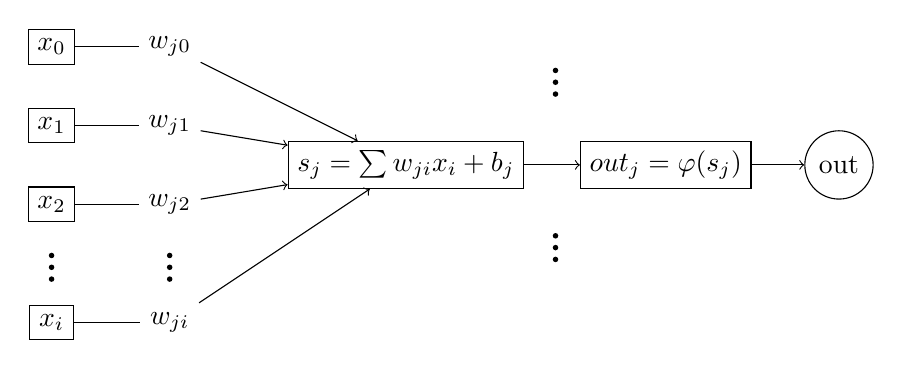
\begin{tikzpicture}
    \tikzstyle{rectangle_style}=[rectangle, draw]
    \tikzstyle{dividedrectangle_style}=[draw, rectangle split, rectangle split parts=2, rotate = 90, minimum height = 15mm, minimum width = 10mm]
    
    % neuron i
    \foreach \x in {0,...,2}
      \draw node at (0, -\x) [rectangle_style] (neuron_i_\x) {$x_\x$};
    \foreach \x in {1,...,3}
      \fill (0, -2.5 - \x*0.15) circle (1pt);
    \draw node at (0, -3.5) [rectangle_style] (neuron_i_3) {$x_i$};
    
    % w_ji
    \foreach \x in {0,...,2}
      \draw node at (1.5, -\x) [] (w_ji_\x) {$w_{j\x}$};
    \draw node at (1.5, -3.5) [] (w_ji_i) {$w_{ji}$};
    \foreach \x in {1,...,3}
      \fill (1.5, -2.5 - \x*0.15) circle (1pt);
    
    % neuron sum
    \draw node at (4.5, -1.5) [rectangle_style] (neuron_sum) {
      $s_j = \sum {w_{ji}x_i+b_j}$
    };
    \draw node at (7.8, -1.5) [rectangle_style] (neuron_act) {
      $out_j = \varphi (s_j)$
    };
    \foreach \x in {1,...,3}
      \fill (6.4, -2.25 - \x*0.15) circle (1pt);
    \foreach \x in {1,...,3}
      \fill (6.4,  - 0.15 - \x*0.15) circle (1pt);
    
    % output
    \node at (10, -1.5) [circle, draw] (output) {out};    

    
    % connect: y_i -> w_ji
    \foreach \i in {0,...,2}
      \path[-] (neuron_i_\i) edge node[] {} (w_ji_\i);
    \path[-] (neuron_i_3) edge node[] {} (w_ji_i);
    
    % connect: w_ji -> neuron j
    \foreach \i in {0,...,2}
      \path[->] (w_ji_\i) edge node[] {} (neuron_sum);
    \path[->] (w_ji_i) edge node[] {} (neuron_sum);
    
     % connect: neuron sum  -> neuron act
     \path[->] (neuron_sum) edge node[above, midway] {$ $} (neuron_act);

    % connect: neuron act -> output
    \path[->] (neuron_act) edge node[above, midway] {$ $} (output);

    
  \end{tikzpicture}
\caption{Схема искусственного нейрона} \label{simple-neuron}
\end{figure}

Множества нейронов формируют слои, слои в свою очередь формируют нейронную сеть. Входной слой получает данные, обрабатывает и передает нейронам скрытого слоя. Аналогично срабатывет каждый последующий слой вплоть до выходного. 

\tikzset{%
every neuron/.style={
  circle,
  draw,
  minimum size=1cm
},
neuron missing/.style={
  draw=none, 
  scale=4,
  text height=0.333cm,
  execute at begin node=\color{black}$\vdots$
},
}
\begin{figure}[H]
  \centering
\begin{tikzpicture}[x=1.5cm, y=1.5cm, >=stealth]

\foreach \m/\l [count=\y] in {1,2,3,missing,4}
\node [every neuron/.try, neuron \m/.try] (input-\m) at (0,2.5-\y) {};

\foreach \m [count=\y] in {1,missing,2}
\node [every neuron/.try, neuron \m/.try ] (hidden-\m) at (2,2-\y*1.25) {};

\foreach \m [count=\y] in {1,missing,2}
\node [every neuron/.try, neuron \m/.try ] (output-\m) at (4,1.5-\y) {};

\foreach \l [count=\i] in {1,2,3,n}
\draw [<-] (input-\i) -- ++(-1,0)
  node [above, midway] {$I_\l$};

\foreach \l [count=\i] in {1,k}
\node [above] at (hidden-\i.north) {$H_\l$};

\foreach \l [count=\i] in {1,p}
\draw [->] (output-\i) -- ++(1,0)
  node [above, midway] {$O_\l$};

\foreach \i in {1,...,4}
\foreach \j in {1,...,2}
  \draw [->] (input-\i) -- (hidden-\j);

\foreach \i in {1,...,2}
\foreach \j in {1,...,2}
  \draw [->] (hidden-\i) -- (output-\j);

\foreach \l [count=\x from 0] in {Входной, Скрытый, Выходной}
\node [align=center, above] at (\x*2,2) {\l \\ слой};
\end{tikzpicture}
\caption{Схема простой нейронной сети} \label{simple-network}
\end{figure}

\subsubsection{Активационная функция}
\label{sec:activation}
Взвешенная сумма входов представляет собой линейную комбинацию входов, из чего следует, что независимо от количества слоев, значения выходного слоя зависят только от входов первого слоя. 
Активационная функция нейрона обеспечивает нормализацию посчитанной суммы и нелинейность нейронной сети. Для многих моделей нейронных сетей также требуется, чтобы активационная функция была монотонной и непрерывно-дифференцируемой на всей области определения.

Существует большое количество функций активации. Наиболее распространенные из них представлены в табл. \ref{actvs}.

\pgfplotsset{
  every axis plot/.append style={
    line width=3pt
  }
}

\begin{table}[H]
  \centering
  \caption{Популярные активационные функции}\label{actvs}
  \begin{tabular}{|c|c|c|}
    \hline    
    \hyperlink{name}{Название} & \hyperlink{func}{Функция} & \hyperlink{chart}{Вид}\\
    \hline
    Сигмоидная &  \resizebox{0.2\hsize}{!}{$\sigma(x)=\frac{1}{1+e^{-x}}$}
    & 
    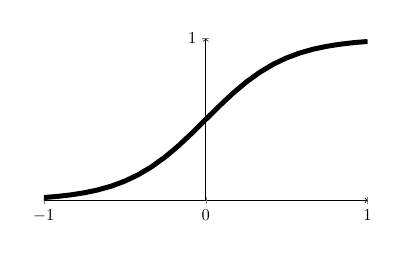
\begin{tikzpicture}[baseline={(0,0.8)}, scale=0.6]      
      \begin{axis}[
        axis equal image,
        axis lines=middle,
        axis line style={->},
        x label style={at={(axis description cs:0.5,-0.1)},anchor=north},
        y label style={at={(axis description cs:-0.1,.5)},rotate=90,      anchor=south},
        extra x ticks=0,
        % extra y ticks=1,
        ymin=0,ymax=1,
        ytick={0, 1},
        xtick={-1, 0, 1}
        ]
        \addplot[domain=-1:1, variable=\x] ({\x},{1/(1+exp(-4*\x))});
      \end{axis}      
    \end{tikzpicture}
   
    \\
    \hline
    Гиперболический тангенс 
    &
    \resizebox{0.2\hsize}{!}{$f(x)=\frac{e^x-e^{-x}}{e^x+e^{-x}}$}
    & 
    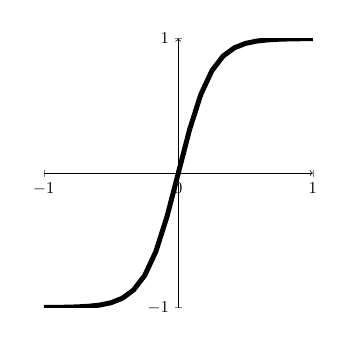
\begin{tikzpicture}[baseline={(0,1.5)},scale=0.6]
      \begin{axis}[
        axis equal image,
        axis lines=middle,
        axis line style={->},
        x label style={at={(axis description cs:0.5,-0.1)},anchor=north},
        y label style={at={(axis description cs:-0.1,.5)},rotate=90,      anchor=south},
         extra x ticks=0,  
        % extra y ticks=1,
        ymin=-1,ymax=1,
        ytick={-1, 0, 1},
        xtick={-1, 0, 1}
        ]
        \addplot[domain=-1:1, variable=\x]({\x},{tanh(4*\x)});
      \end{axis}      
    \end{tikzpicture} 
    \\
    \hline
    ReLU & \resizebox{0.2\hsize}{!}{$f(x) =\begin{cases}
    0, & x<0 \\ 
    x, & x \geq 0.
    \end{cases}$} & 
    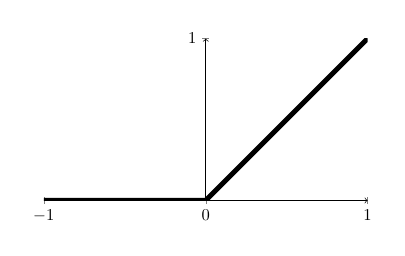
\begin{tikzpicture}[baseline={(0,0.8)},scale=0.6]
      \begin{axis}[
        axis equal image,
        axis lines=middle,
        axis line style={->},
        x label style={at={(axis description cs:0.5,-0.1)},anchor=north},
        y label style={at={(axis description cs:-0.1,.5)},rotate=90,anchor=south},
         extra x ticks=0,  
        % extra y ticks=1,
        ymin=0,ymax=1,
        ytick={0, 1},
        xtick={-1, 0, 1}
        ]
        \addplot[domain=-1:1, variable=\x]({\x},{ifthenelse(\x<0,0,\x)});
      \end{axis}      
    \end{tikzpicture}
    \\
    \hline
  \end{tabular}
\end{table}

\subsubsection{Глубокое машинное обучение}
Глубокое обучение (Deep Learning) - область машинного обучения, в которой для решения задач используются глубокие нейронные сети. Под глубокими нейронными сетями понимают сети с большим количеством скрытых слоев. 

\subsubsection{Обучение нейронных сетей}
Под обучением нейронных сетей подразумевают настройку значений весов связей для эффективного решения поставленной задачи. Изначально, веса устанавливаются случайно. Затем, в процессе прогона через сеть тестовых данных, веса корректируются так, чтобы в конечном итоге сеть выдавала правильные ответы. 

Существует несколько способов обучения нейронных сетей:

Обучение с учителем – 
% это такой тип обучения, в котором известны и входные, и выходные вектора сети. Имеются пары вход + выход — известные условия задачи и решение. В процессе обучения сеть меняет свои параметры и учится давать нужное отображение X→Y. Нейросеть учится выдавать результаты, которые нам уже известны. За счет способности к обобщению сетью могут быть получены новые результаты, если подать на вход вектор, который не встречался при обучении.
Обучение с подкреплением -  

Обучение без учителя - 

Генетические алгоритмы обучения - 


\subsubsection{Сверточные нейронные сети}
Сверточные нейронные сети (Convolutional Neural Network) активно применяются в задачах распознавания образов. 
% В сверточных сетях очень популярна активационная функция ReLU.
\subsection{Применение нейронных сетей в задачах распознавания изображений}
???

TensorFlow - многофункциональный фреймворк для машинного обучения с открытым исходным кодом

Keras ???

???
\clearpage